\documentclass[a4j,11pt,dvipdfmx]{jsarticle}
\usepackage{float}
\usepackage{array}
\usepackage{titlesec}
\usepackage[dvipdfmx]{graphicx}
\usepackage{graphicx}
\usepackage{url}

\titleformat*{\section}{\bfseries}
\titleformat*{\subsection}{\bfseries}

\makeatletter
  \renewcommand{\section}{%
    \@startsection{section}{1}{\z@}%
    {0.4\Cvs}{0.1\Cvs}%
    {\normalfont\headfont\raggedright}}
\makeatother

\makeatletter
  % sectionの下マージンを小さく
  \renewcommand{\subsection}{%
    \@startsection{subsection}{1}{\z@}%
    {0.1\Cvs}{0.1\Cvs}%
    {\normalfont\headfont\raggedright}}
\makeatother

\renewcommand{\thesubsection}{\thesection-\arabic{subsection}.}


%---------------------------------------------------
% ページの設定
%---------------------------------------------------
\setlength{\textwidth}{160truemm}
\setlength{\textheight}{250truemm}
\setlength{\topmargin}{-4.5truemm}
\setlength{\oddsidemargin}{0.5truemm}
\pagestyle{empty}
\setlength{\headheight}{0truemm}
\setlength{\parindent}{1zw}
\newcolumntype{b}{!{\vrule width 1pt}}
\newcommand{\bhline}{\noalign{\hrule height 1pt}}   


\begin{document}
提出日: 20xx年xx月xx日
\begin{center}
\huge{実験計画書}
\end{center}
\begin{flushright}
\end{flushright}
\begin{table}[H]
  \centering
  \begin{tabular}{bp{15.5truecm}b}
  \bhline
  \large{\bf{}}
  \\ \bhline
\end{tabular}
\end{table}


%%%%%%%%%%%%%%%%%%%%%%%%%%%%%%%%%%%%%%%%%%%%%%%%%
%%%%%%%%%%%%%%%%%%%%%%%%%%%%%%%%%%%%%%%%%%%%%%%%%
%%%%%%%%%%%%%%%%%%%%%%%%%%%%%%%%%%%%%%%%%%%%%%%%%
\section{技術的・社会的な背景とシステムの目的}\label{sec:intro}
\begin{table}[H]
\vspace{-1em}
\centering
\begin{tabular}{bp{15.5truecm}b}
\bhline
\subsection{技術的・社会的な課題や要求}
	\\ \bhline
\subsection{類似のシステム}
	 \\ \bhline
\subsection{システムの目的と独自性}
	\\ \bhline
\end{tabular}
\end{table}

%%%%%%%%%%%%%%%%%%%%%%%%%%%%%%%%%%%%%%%%%%%%%%%%%
%%%%%%%%%%%%%%%%%%%%%%%%%%%%%%%%%%%%%%%%%%%%%%%%%
%%%%%%%%%%%%%%%%%%%%%%%%%%%%%%%%%%%%%%%%%%%%%%%%%
\section{システムの概要}\label{sec:about_system}
\begin{table}[H]
\vspace{-1em}
\centering
\begin{tabular}{bp{15.5truecm}b}
\bhline
\subsection{システム全体の構成}
	
	\\ \bhline
\subsection{1つ目の要素システムの構成}
	
	 \\ \bhline
\subsection{音通信システムの構成}
音通信システムの構成図を図\ref{fig:sound_composition}に,動作の流れを図\ref{fig:flow_sound_tx},図\ref{fig:flow_sound_rcv}に示す.
送信側Arduinoで光の受信によって取得した4進数の数列を音に変換し,ダイナミックスピーカーから音波を出力する.
このとき出力する音波は,取得した数列を2シンボルずつに分け,各2シンボルに対応した16個の周波数の音波である.
ダイナミックスピーカーから出力された音波は受信側Arduinoに接続されたマイクに入力される.
入力された音波からその周波数を検知し,周波数に対応する2桁の4進数を受信側Arduinoで取得する.

	 \\ \bhline
\subsection{$n$つ目の要素システムの構成}
	
	 \\ \bhline
\end{tabular}
\end{table}

\begin{figure}[h]
    \centering
    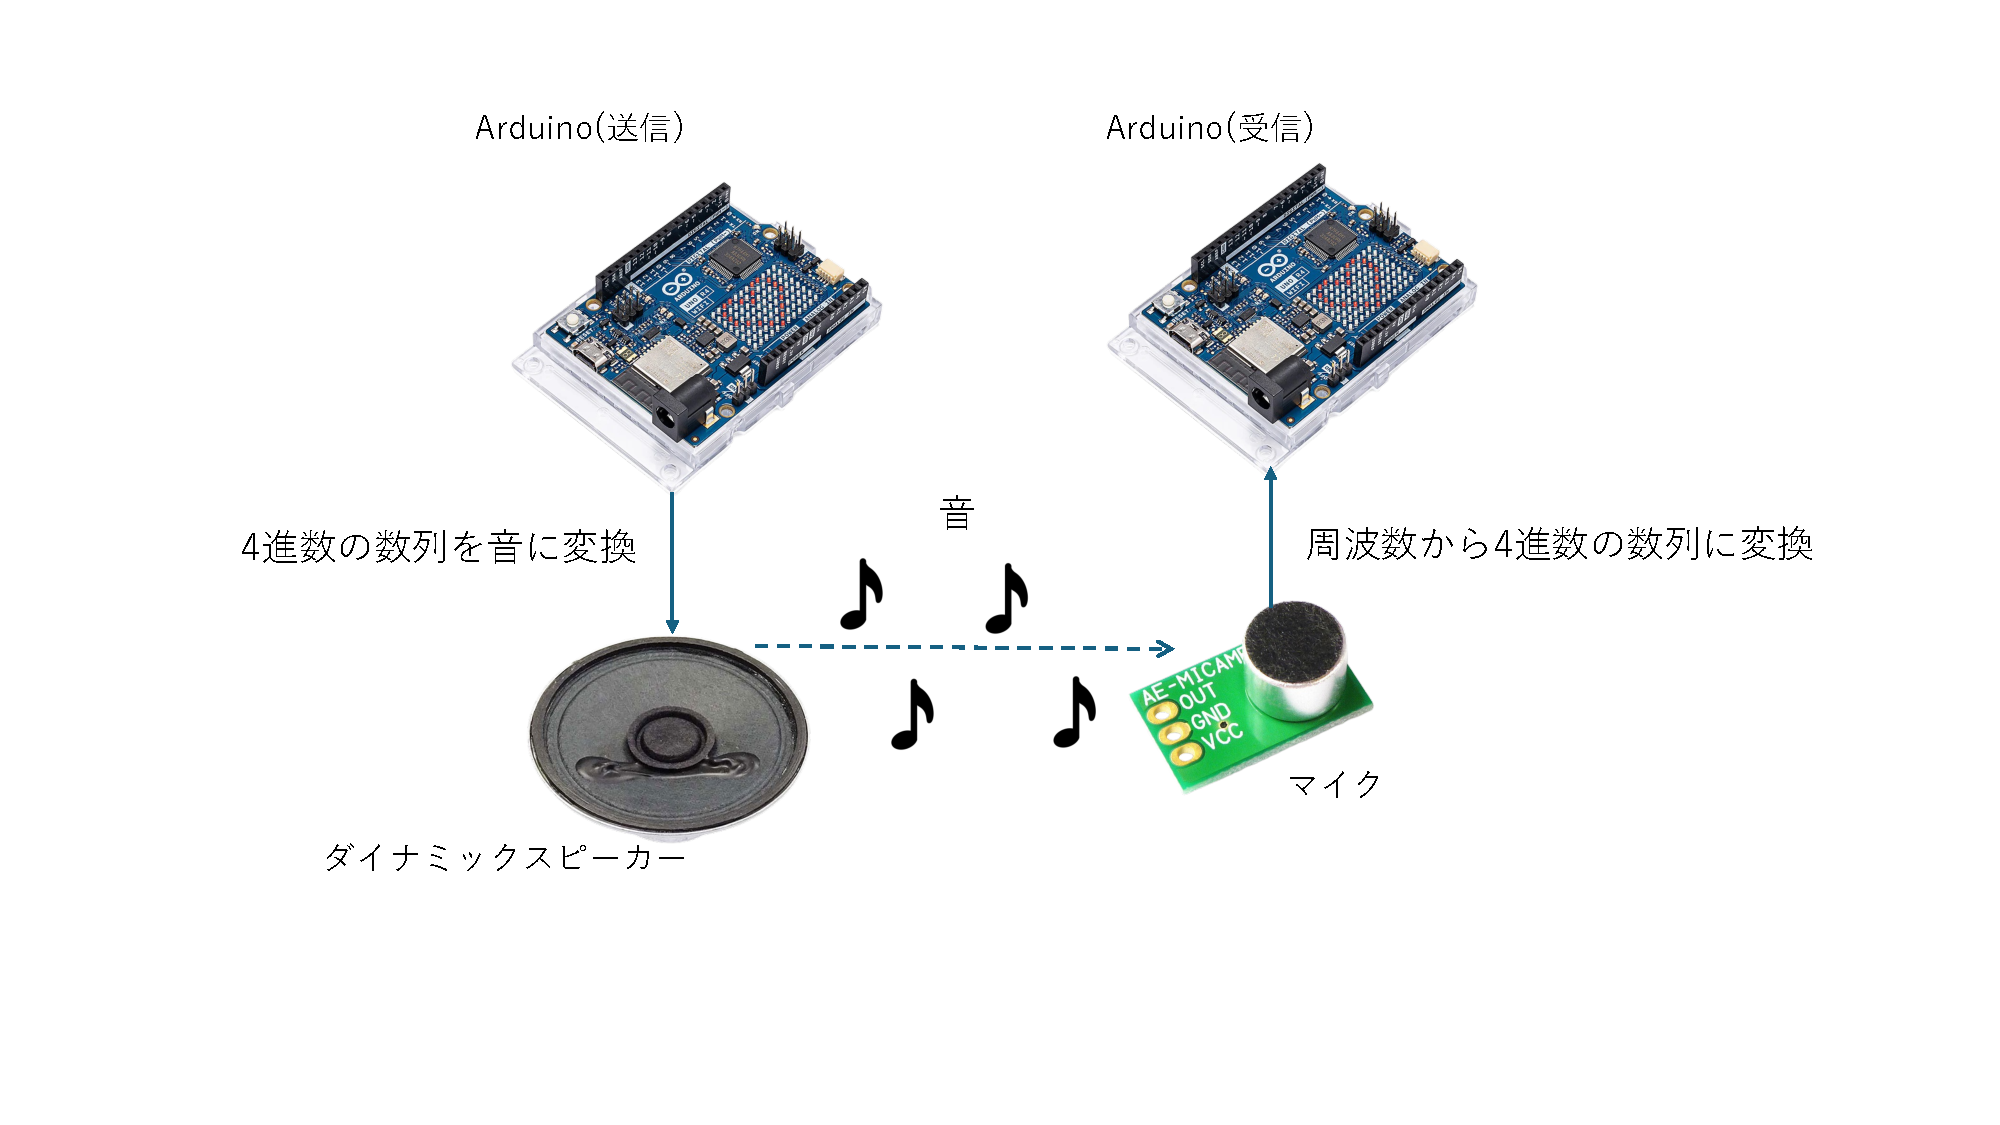
\includegraphics[width=160mm]{../img/sound_composition.pdf}
    \caption{音通信システムの構成図}
    \label{fig:sound_composition}
\end{figure}

\begin{figure}[h]
    \centering
    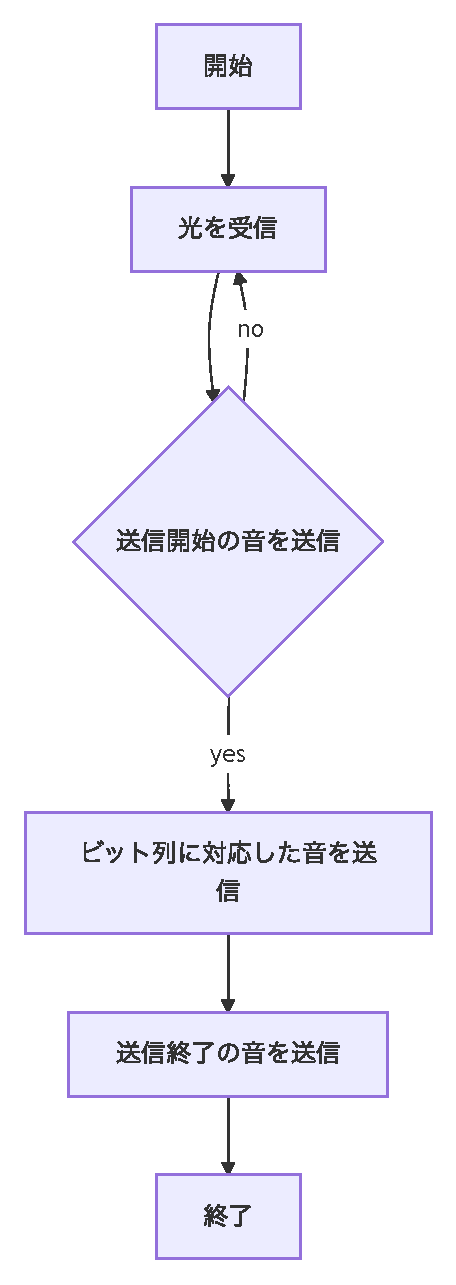
\includegraphics[width=40mm]{../img/flow_sound_tx-1.pdf}
    \caption{音通信システム(送信側)のフローチャート}
    \label{fig:flow_sound_tx}
\end{figure}

\begin{figure}[h]
    \centering
    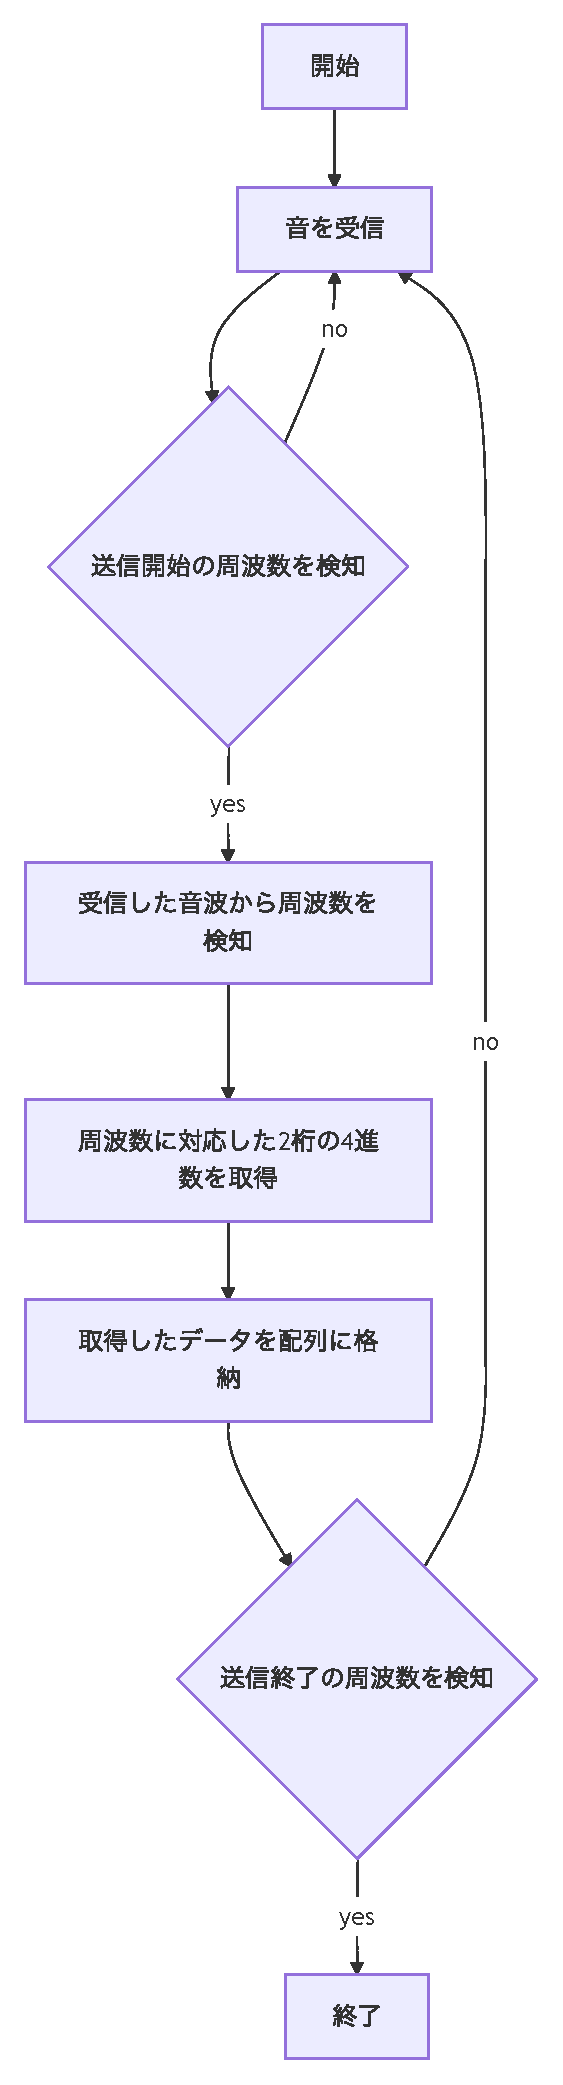
\includegraphics[width=60mm]{../img/flow_sound_rcv-1.pdf}
    \caption{音通信システム(受信側)のフローチャート}
    \label{fig:flow_sound_rcv}
\end{figure}


%%%%%%%%%%%%%%%%%%%%%%%%%%%%%%%%%%%%%%%%%%%%%%%%%
%%%%%%%%%%%%%%%%%%%%%%%%%%%%%%%%%%%%%%%%%%%%%%%%%
%%%%%%%%%%%%%%%%%%%%%%%%%%%%%%%%%%%%%%%%%%%%%%%%%
\clearpage
\section{必要な作業}\label{sec:tasks}
\begin{table}[H]
\vspace{-1em}
\centering
\begin{tabular}{bp{15.5truecm}b}
\bhline
\subsection{1つ目の要素システムを構築する作業}
% 光を用いた通信システムでは,8個のLEDの色のパターンを利用してデータの送受信を行う.
% このシステムはLEDを8個並べて全消灯から全点灯で8bitを表すため,各LEDに照度センサを対応させ,そのビット列を判断する.
% まずArduinoにセンサを各ピンに接続し,LEDの光を受け取る回路を組む.
% 次にセンサから光を受け取ると0または1を返すプログラムを作成し,8つのセンサの0または1の情報を結合してビット列に直す.
% そして,直したビット列からasciiコードに対応した文字に変換する.
% 	 \\ \bhline
\subsection{音通信システムを構築する作業}
% 音を用いた通信システムでは,低いドから高いドまでの8つの音程を利用してデータの送受信を行う.
% まず光の受信によって変換した文字をasciiコードから8bitのビット列に変換する.
% このビット列を4bitずつ半分に分け,各4bitに対応した音を鳴らすことで1文字を表現する.
% このために,Arduinoにスピーカを接続し,分けた4bitに対応する音を出力するプログラムを作成する
\begin{itemize}
  \item Arduinoと抵抗器,ダイナミックスピーカを接続し音波を出力可能な回路をブレッドボード上に組む
    \begin{itemize}
      \item Arduinoのデジタルピンと330 $\Omega$の抵抗器,ダイナミックスピーカーを直列に接続
    \end{itemize}
  \item 受信した数列に応じて音波を送信するプログラムを作成する
    \begin{itemize}
      \item 4 bitの4進数の数列を受信する
      \item 17個の音程を用意し,1個は開始と終了の合図に,他の16個は受信した数列を2 シンボル $\times$ 2個に分けた各2 シンボルを表す為に設定する
      \item 受信した数列に対応する音程(周波数)の音波をスピーカーから出力する
    \end{itemize}
  \item マイクと抵抗器,Arduinoを接続し音波を入力可能な回路をブレッドボード上に組む
  \item 入力した音波の周波数を特定し,対応する数値を取得するプログラムを作成
    \begin{itemize}
      \item 受信した波の頂点を検知し,その周期から周波数を得る
      \item 得た周波数に対応する数値(2シンボル)を取得する
    \end{itemize}
  \item 取得した数値からテキストを復元
\end{itemize}

	 \\ \bhline
\subsection{$n$つ目の要素システムの構成}

	 \\ \bhline
\subsection{全体のシステム(要素システムの結合)}
	
	\\ \bhline
\end{tabular}
\end{table}

%%%%%%%%%%%%%%%%%%%%%%%%%%%%%%%%%%%%%%%%%%%%%%%%%
%%%%%%%%%%%%%%%%%%%%%%%%%%%%%%%%%%%%%%%%%%%%%%%%%
%%%%%%%%%%%%%%%%%%%%%%%%%%%%%%%%%%%%%%%%%%%%%%%%%
\section{担当者割り当て}\label{sec:assignment}
各作業の担当者を図\ref{fig:wbs}に示す.
\begin{figure}[h]
    \centering
    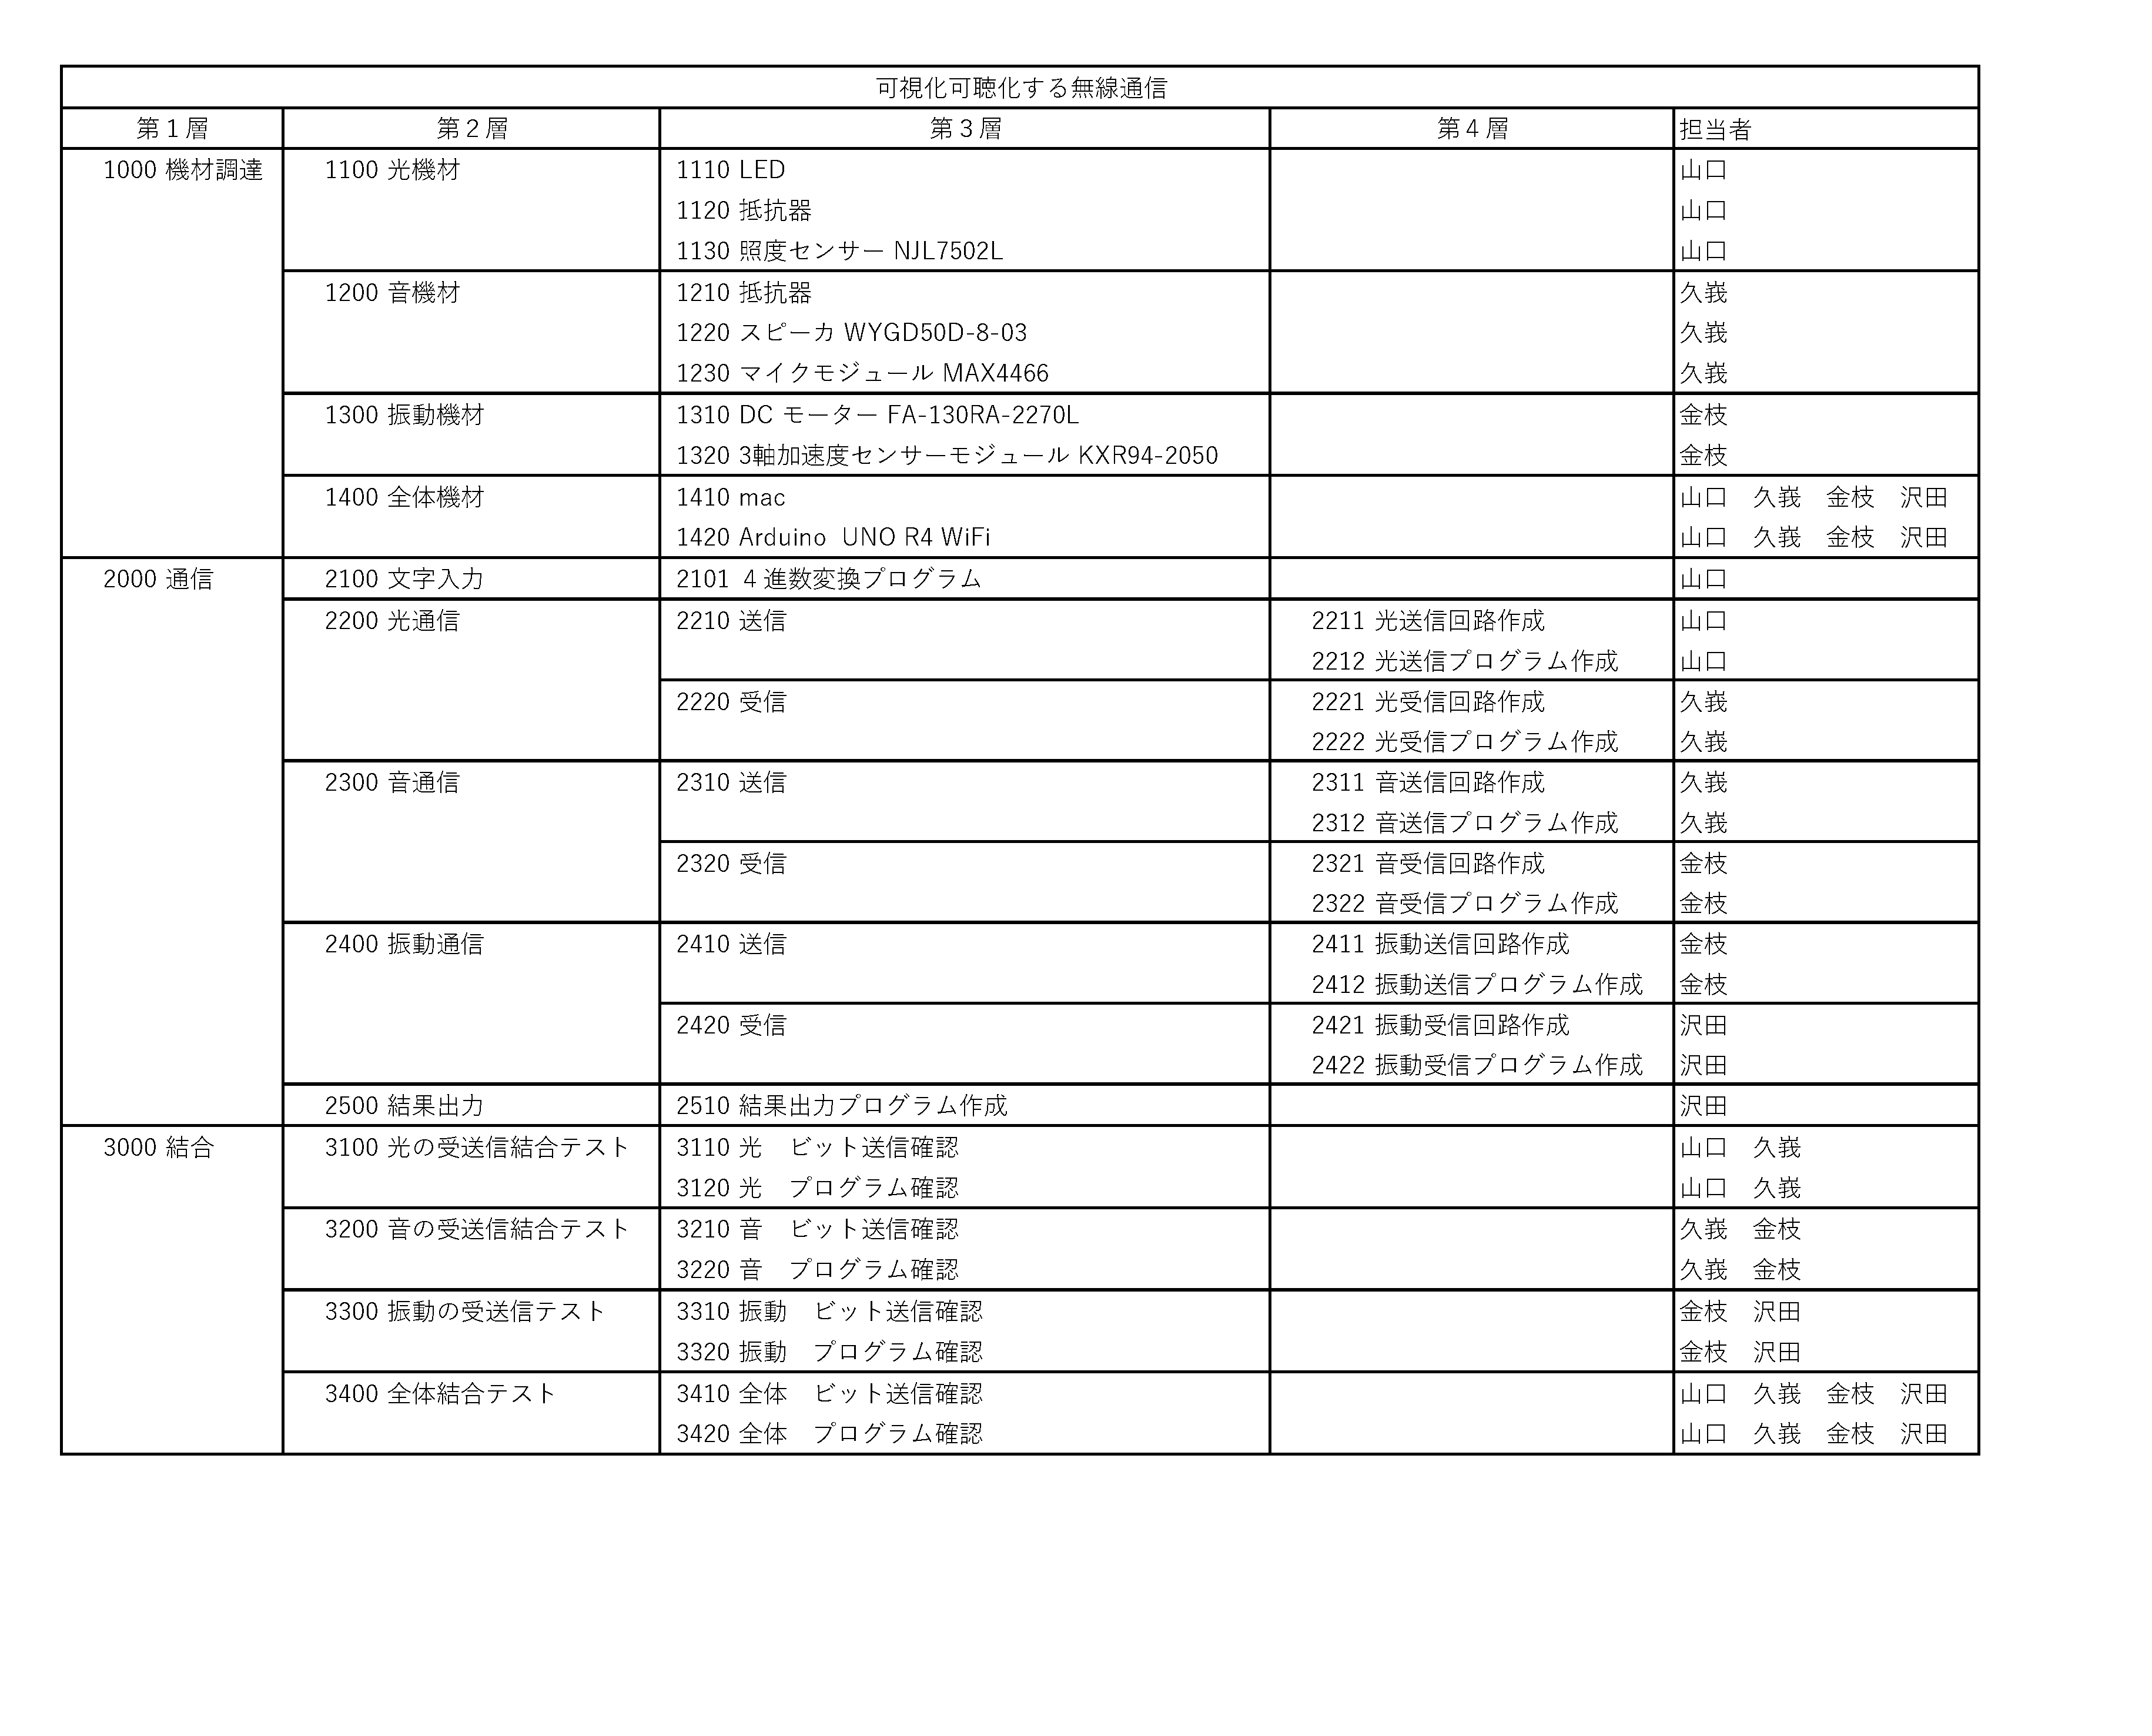
\includegraphics[width=\textwidth]{../img/wbs.pdf}
    \caption{WBS図と担当者割当}
    \label{fig:wbs}
\end{figure}


%%%%%%%%%%%%%%%%%%%%%%%%%%%%%%%%%%%%%%%%%%%%%%%%%
%%%%%%%%%%%%%%%%%%%%%%%%%%%%%%%%%%%%%%%%%%%%%%%%%
%%%%%%%%%%%%%%%%%%%%%%%%%%%%%%%%%%%%%%%%%%%%%%%%%
\section{スケジュール}\label{sec:schedule}
本システムのスケジュールを図\ref{fig:gantt}のガントチャートで示す.

\begin{figure}[h]
    \centering
    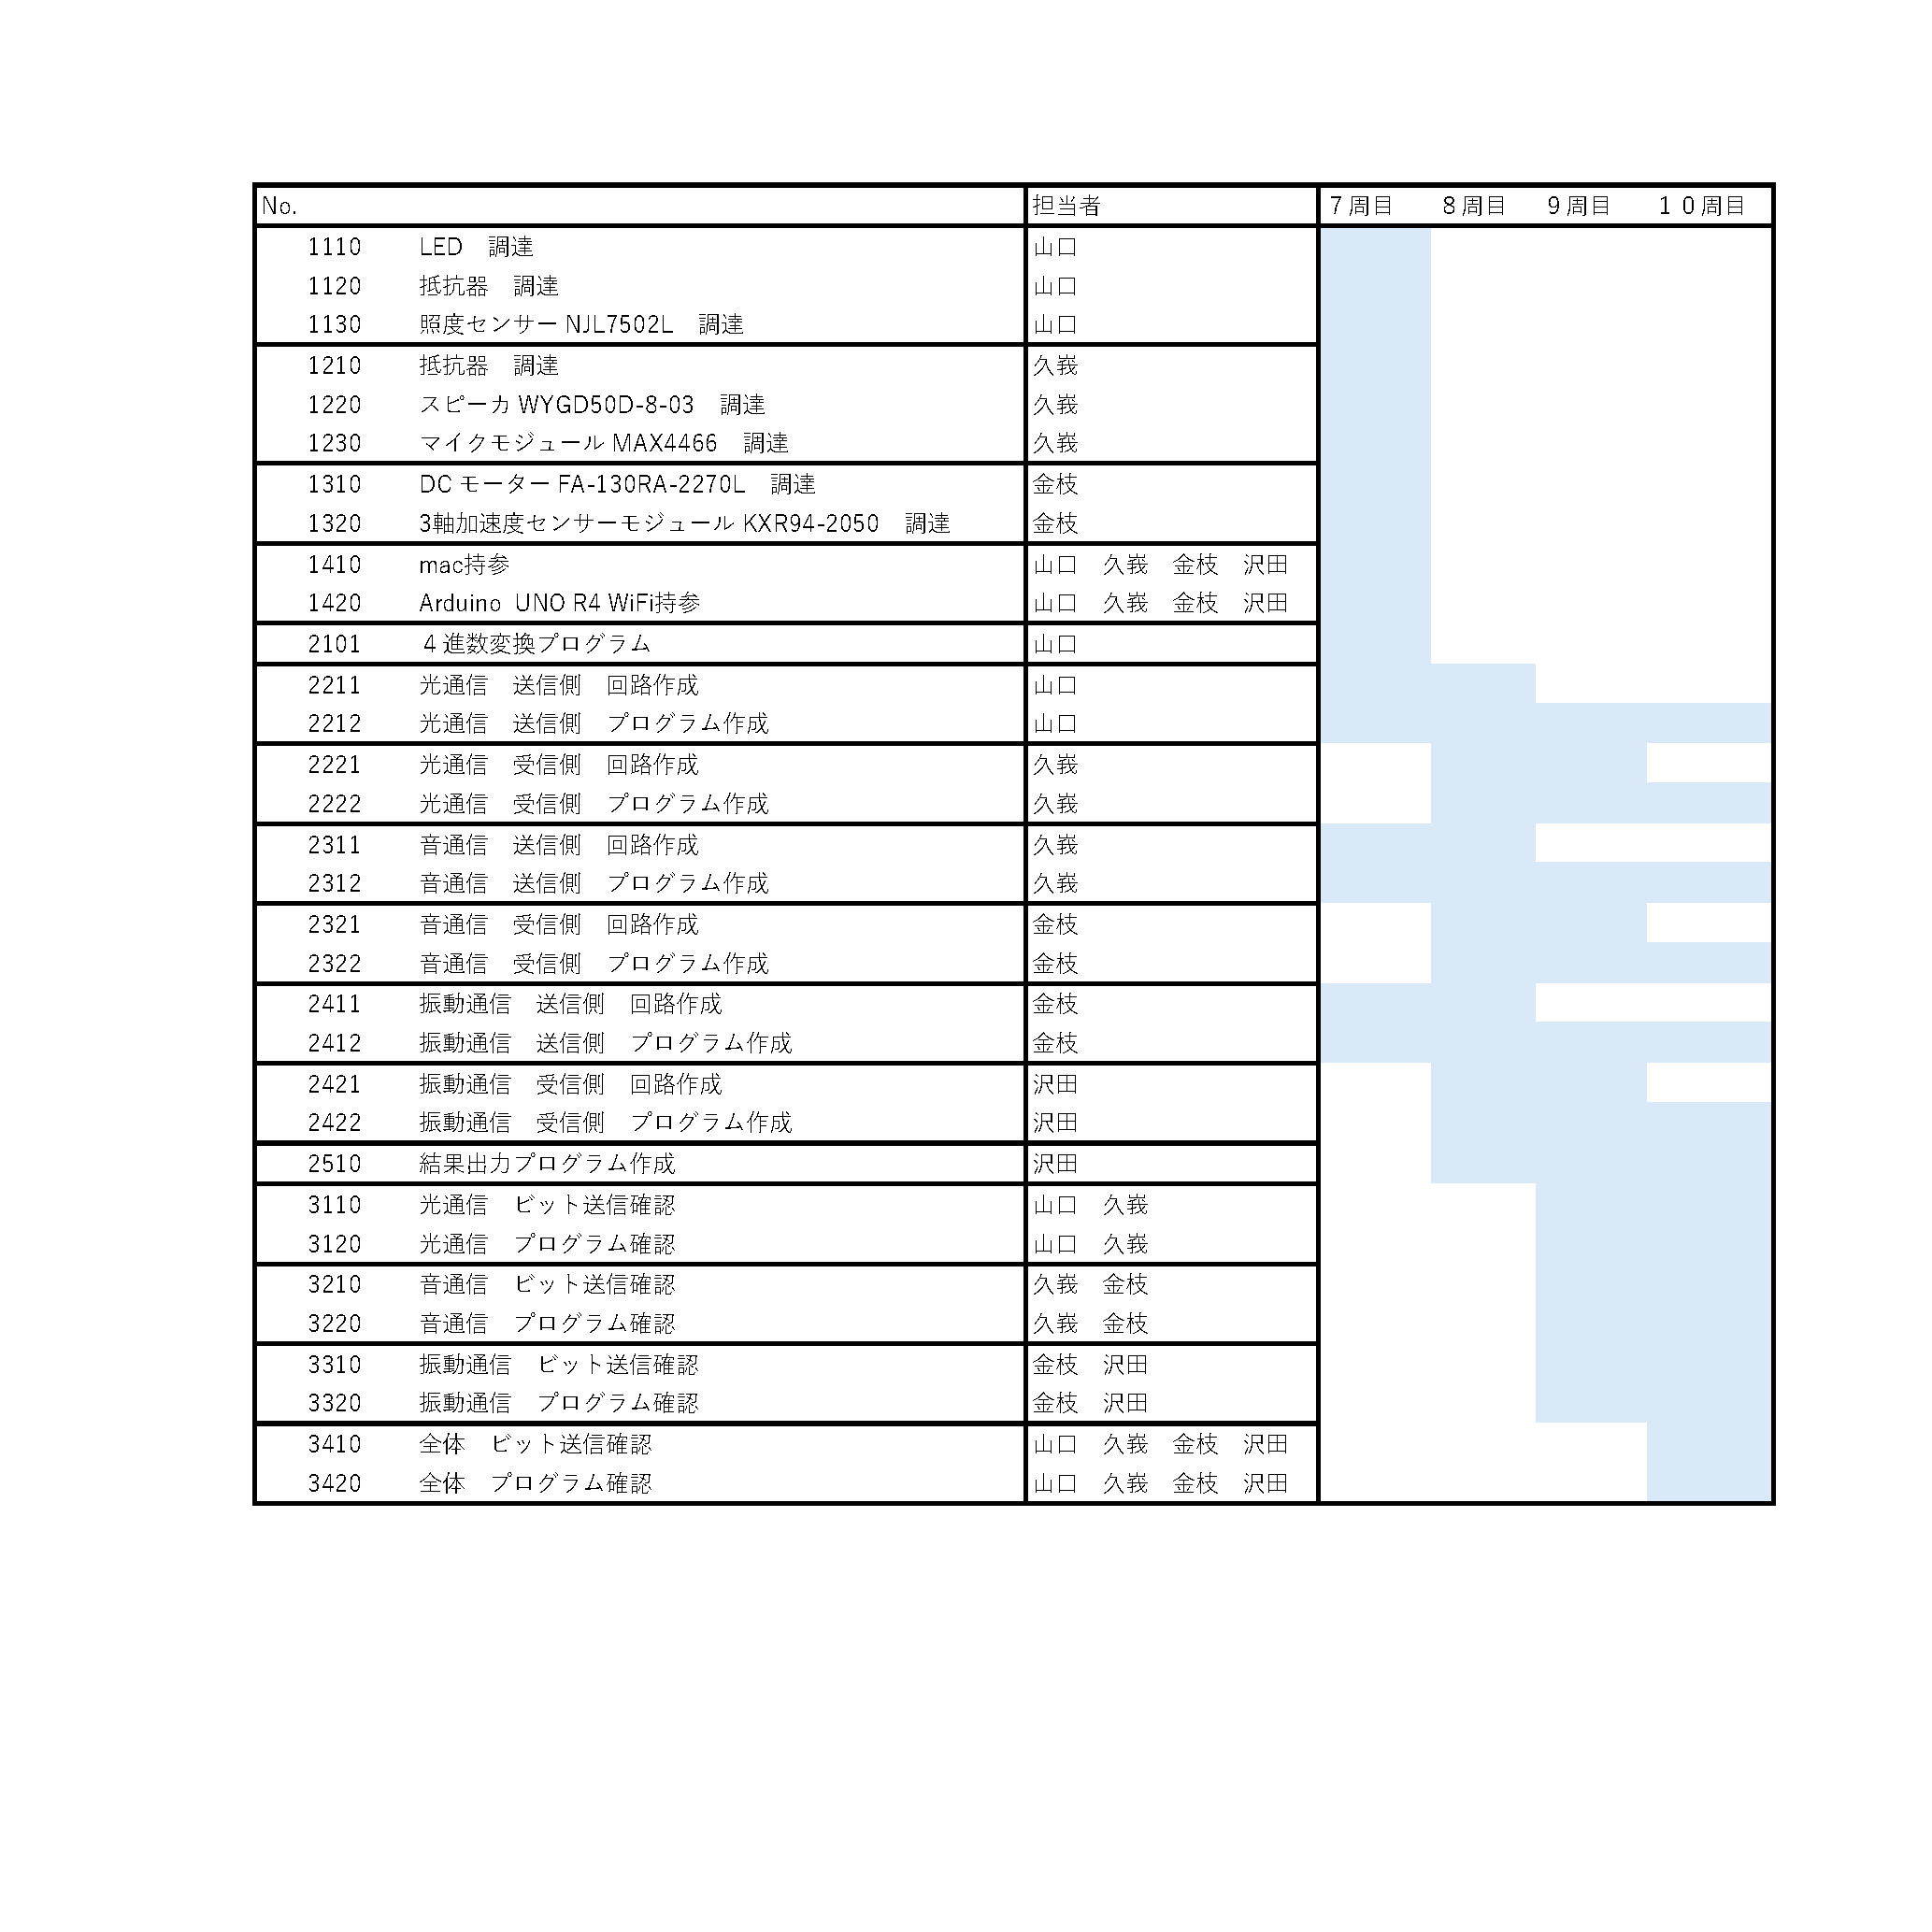
\includegraphics[width=\textwidth]{../img/ganttchart.pdf}
    \caption{各作業のスケジュール}
    \label{fig:gantt}
\end{figure}


%%%%%%%%%%%%%%%%%%%%%%%%%%%%%%%%%%%%%%%%%%%%%%%%%
%%%%%%%%%%%%%%%%%%%%%%%%%%%%%%%%%%%%%%%%%%%%%%%%%
%%%%%%%%%%%%%%%%%%%%%%%%%%%%%%%%%%%%%%%%%%%%%%%%%
\section{必要な機材}\label{sec:equipment}
本システムの構築に必要な機材を表\ref{table:equipment}に示す.
\begin{table}[h]
    \centering
    \caption{必要な機材}
    \label{table:equipment}
    \begin{tabular}{|l|c|c|c|c|}
  \hline
  機材名 &仕様 &数量 &調達方法 &費用(円)  \\ \hline \hline
  Arduino Uno R4 WiFi &ABX00087 &2 &持参 &0 \\ \hline
  ブレッドボードEIC-102J &0165-41-4-1020 &2 &持参 &0 \\ \hline
  ダイナミックスピーカー &WYGD50D-8-03 &1 &購入 &240 \\ \hline
  マイクアンプモジュール &AE-MICAMP &1 &購入 &500 \\ \hline
  炭素被膜抵抗 &330$\Omega$ &2 &持参 &0 \\ \hline
    \end{tabular}  
\end{table}


%\newpage
%%%%%%%%%%%%%%%%%%%%%%%%%%%%%%%%%%%%%%%%%%%%%%%%%
%%%%%%%%%%%%%%%%%%%%%%%%%%%%%%%%%%%%%%%%%%%%%%%%%
%%%%%%%%%%%%%%%%%%%%%%%%%%%%%%%%%%%%%%%%%%%%%%%%%
\section{システムの評価指標と具体的な数値目標}\label{sec:evaluation}
% 音の受信について,音がなってからLEDが点灯するまでの応答時間を1秒以下にすることを目標とする.
% 人間がデータ入力をしてから応答があるまでにラグを感じずに作業できるためである\cite{ref:user_reaction}.
% 光の受信について,照度センサが光を検知してテキストが出力されるまでにかかる時間を100 msに抑えることを目標とする.
% これはLEDの光の反射から傾斜角を計測する傾斜センサの応答時間が100msほどであるからである\cite{ref:keisha}.
音の送信における評価指標として,通信距離と通信精度,通信速度を評価する.
初めに通信距離について評価指標を設定する.
屋内でスピーカからのサイレン音をスマートフォンを用いて受信する実験では通信距離が10 mを超えても適切に通信が可能であると報告があり\cite{ref:tone}\cite{ref:tone2}.今回の音程の差による通信について,通信可能距離=10 mを目標とする.
\par
次に通信精度について評価指標を設定する.
音を連続で鳴らすと,一つ前になった音が遅延や反射によってその後に鳴った音と干渉するシンボル間干渉(ISI)が生じる可能性がある.
ISIを軽減,防止するために,シンボル間に通信しない間隔のガードインターバル(GI)を設ける.
通信の際GIをシンボル長の25\%にすることで干渉を防ぎつつ効率の良い通信が可能となる\cite{ref:GI}.
また,デジタル通信では,伝送品質の指標としてビット誤り率(BER)が用いられる\cite{ref:BER}.
BERは誤ったビットを受信する確率で,送信されたビット数$N_t$と誤って受信したビット数$N_e$を用いて式\ref{eq:BER}で表される.


\begin{equation}
  \label{eq:BER}
  BER = \frac{N_e}{N_t}
\end{equation}

% このBERは通常の誤り訂正により$BER<10^{-3}$に抑えられることが報告されているため\cite{ref:BER_less},音通信システムにおける通信精度について,$BER<10^{-3}$を目標とする.
データのビット値を音のオンオフによって符号化した音響通信の例では,雑音が通信音量以下だとBERは約2\%で,雑音が大きい環境だとBERが10\%を超えたという結果があり\cite{ref:mobile_sound},これを踏まえ音通信システムにおける通信精度について,$BER<10^{-1}$を目標とする.
\par
次に通信速度について評価指標を設定する.
先ほどの研究\cite{ref:mobile_sound}では2進数データを4bitのブロックに区切り,各ブロックを0.4 sの音で通信した.
この通信速度を計算すると10 bpsとなり,この速度でBERが約2\%であるため,10 bpsで適切な通信が可能だと考える.
また,この研究と類似した条件で音通信システムの速度を計算すると音長0.3 sで10.$\dot{6}$bpsとなり軽微な高速化が図れる.
よって,音通信システムにおける通信速度について,bps=10 sを目標とする.
\begin{thebibliography}{99}
  % \bibitem{ref:user_reaction}
  % Ben Shneiderman, Catherine Plaisant,Designing the User Interface: Strategies for Effective Human-Computer Interaction,Addison-Wesley,Vol.4,2004

  % \bibitem{ref:kenchi}
  % 水知 力,梅林 健太,Janne J. Lehtom\"\a ki,Miguel L\'opez-Bena\'\i tez,鈴木 康夫,周波数利用観測のための誤警報除去法のパラメータ設計に関する一検討,電子情報通信学会,2016

%   \bibitem{ref:keisha}
%   下尾 浩正,南部 幸久,寺村 正広,ニューラルネットワーク比較器を用いた傾斜センサによる応答時間の短縮,電気学会論文誌,Vol.139,No.9,pp.310-316,2019

  \bibitem{ref:tone}
  小嶋 徹也,鎌田 寛,Udaya PARAMPALLI,楽曲を用いた通信システム,東京工業高等専門学校研究報告書,No.49,2017.
  \bibitem{ref:tone2}
  Youki Sada, Tetsuya Kojima,"Improvement of Emergency Broadcasting System Based on Audio Data Hiding",IEICE Tech. Rep.,Vol.117,No.476,EMM2017-88,pp.55-60,2018.
  \bibitem{ref:GI}
  Md. Zahid Hasan, Mohammad Reaz Hossain, Md. Ashraful Islam, Riaz Uddin Mondal,"Comparative Study of Different Guard Time Intervals to Improve the BER Performance of Wimax Systems to Minimize the Effects of ISI
  and ICI under Adaptive Modulation Techniques over SUI-1 and AWGN Communication Channels",IJCSIS,Vol.6, No.2,pp128-132,2009.
  \bibitem{ref:BER}
  Jia Dong,"Estimation of Bit Error Rate of any digital Communication System",Télécom Bretagne,HAL Open Science,2013.
  \bibitem{ref:mobile_sound}
  大石 智久,「音楽性信号への符号化による携帯端末用音響通信」,三重大学学術機関リポジトリ,2014.
  % \bibitem{ref:BER_less}
  % 久米 達哉,八木 生剛,今井 欽之,山本 学,「ディジタルホログラフィックメモリのBER の向上」,映像情報メディア学会技術報告,Vol.24,No.21,pp31-36,2000.
\end{thebibliography}
\end{document}
